\documentclass{ximera}
\usepackage{amssymb, latexsym, amsmath, amsthm, graphicx, amsthm,alltt,color, listings,multicol,xr-hyper,hyperref,aliascnt,enumitem}
\usepackage{xfrac}

\usepackage{parskip}
\usepackage[,margin=0.7in]{geometry}
\setlength{\textheight}{8.5in}

\usepackage{epstopdf}

\DeclareGraphicsExtensions{.eps}
\usepackage{tikz}


\usepackage{tkz-euclide}
%\usetkzobj{all}
\tikzstyle geometryDiagrams=[rounded corners=.5pt,ultra thick,color=black]
\colorlet{penColor}{black} % Color of a curve in a plot


\usepackage{subcaption}
\usepackage{float}
\usepackage{fancyhdr}
\usepackage{pdfpages}
\newcounter{includepdfpage}
\usepackage{makecell}


\usepackage{currfile}
\usepackage{xstring}




\graphicspath{  
{./otherDocuments/}
}

\author{Claire Merriman}
\newcommand{\classday}[1]{\def\classday{#1}}

%%%%%%%%%%%%%%%%%%%%%
% Counters and autoref for unnumbered environments
% Not needed??
%%%%%%%%%%%%%%%%%%%%%
\theoremstyle{plain}


\newtheorem*{namedthm}{Theorem}
\newcounter{thm}%makes pointer correct
\providecommand{\thmname}{Theorem}

\makeatletter
\NewDocumentEnvironment{thm*}{o}
 {%
  \IfValueTF{#1}
    {\namedthm[#1]\refstepcounter{thm}\def\@currentlabel{(#1)}}%
    {\namedthm}%
 }
 {%
  \endnamedthm
 }
\makeatother


\newtheorem*{namedprop}{Proposition}
\newcounter{prop}%makes pointer correct
\providecommand{\propname}{Proposition}

\makeatletter
\NewDocumentEnvironment{prop*}{o}
 {%
  \IfValueTF{#1}
    {\namedprop[#1]\refstepcounter{prop}\def\@currentlabel{(#1)}}%
    {\namedprop}%
 }
 {%
  \endnamedprop
 }
\makeatother

\newtheorem*{namedlem}{Lemma}
\newcounter{lem}%makes pointer correct
\providecommand{\lemname}{Lemma}

\makeatletter
\NewDocumentEnvironment{lem*}{o}
 {%
  \IfValueTF{#1}
    {\namedlem[#1]\refstepcounter{lem}\def\@currentlabel{(#1)}}%
    {\namedlem}%
 }
 {%
  \endnamedlem
 }
\makeatother

\newtheorem*{namedcor}{Corollary}
\newcounter{cor}%makes pointer correct
\providecommand{\corname}{Corollary}

\makeatletter
\NewDocumentEnvironment{cor*}{o}
 {%
  \IfValueTF{#1}
    {\namedcor[#1]\refstepcounter{cor}\def\@currentlabel{(#1)}}%
    {\namedcor}%
 }
 {%
  \endnamedcor
 }
\makeatother

\theoremstyle{definition}
\newtheorem*{annotation}{Annotation}
\newtheorem*{rubric}{Rubric}

\newtheorem*{innerrem}{Remark}
\newcounter{rem}%makes pointer correct
\providecommand{\remname}{Remark}

\makeatletter
\NewDocumentEnvironment{rem}{o}
 {%
  \IfValueTF{#1}
    {\innerrem[#1]\refstepcounter{rem}\def\@currentlabel{(#1)}}%
    {\innerrem}%
 }
 {%
  \endinnerrem
 }
\makeatother

\newtheorem*{innerdefn}{Definition}%%placeholder
\newcounter{defn}%makes pointer correct
\providecommand{\defnname}{Definition}

\makeatletter
\NewDocumentEnvironment{defn}{o}
 {%
  \IfValueTF{#1}
    {\innerdefn[#1]\refstepcounter{defn}\def\@currentlabel{(#1)}}%
    {\innerdefn}%
 }
 {%
  \endinnerdefn
 }
\makeatother

\newtheorem*{scratch}{Scratch Work}


\newtheorem*{namedconj}{Conjecture}
\newcounter{conj}%makes pointer correct
\providecommand{\conjname}{Conjecture}
\makeatletter
\NewDocumentEnvironment{conj}{o}
 {%
  \IfValueTF{#1}
    {\innerconj[#1]\refstepcounter{conj}\def\@currentlabel{(#1)}}%
    {\innerconj}%
 }
 {%
  \endinnerconj
 }
\makeatother

\newtheorem*{poll}{Poll question}
\newtheorem{tps}{Think-Pair-Share}[section]


\newenvironment{obj}{
	\textbf{Learning Objectives.} By the end of class, students will be able to:
		\begin{itemize}}
		{\!.\end{itemize}
		}

\newenvironment{pre}{
	\begin{description}
	}{
	\end{description}
}


\newcounter{ex}%makes pointer correct
\providecommand{\exname}{Homework Problem}
\newenvironment{ex}[1][2in]%
{%Env start code
\problemEnvironmentStart{#1}{Homework Problem}
\refstepcounter{ex}
}
{%Env end code
\problemEnvironmentEnd
}

\newcommand{\inlineAnswer}[2][2 cm]{
    \ifhandout{\pdfOnly{\rule{#1}{0.4pt}}}
    \else{\answer{#2}}
    \fi
}


\ifhandout
\newenvironment{shortAnswer}[1][
    \vfill]
        {% Begin then result
        #1
            \begin{freeResponse}
            }
    {% Environment Ending Code
    \end{freeResponse}
    }
\else
\newenvironment{shortAnswer}[1][]
        {\begin{freeResponse}
            }
    {% Environment Ending Code
    \end{freeResponse}
    }
\fi

\let\question\relax
\let\endquestion\relax

\newtheoremstyle{ExerciseStyle}{\topsep}{\topsep}%%% space between body and thm
		{}                      %%% Thm body font
		{}                              %%% Indent amount (empty = no indent)
		{\bfseries}            %%% Thm head font
		{}                              %%% Punctuation after thm head
		{3em}                           %%% Space after thm head
		{{#1}~\thmnumber{#2}\thmnote{ \bfseries(#3)}}%%% Thm head spec
\theoremstyle{ExerciseStyle}
\newtheorem{br}{In-class Problem}

\newenvironment{sketch}
 {\begin{proof}[Sketch of Proof]}
 {\end{proof}}


\newcommand{\gt}{>}
\newcommand{\lt}{<}
\newcommand{\N}{\mathbb N}
\newcommand{\Q}{\mathbb Q}
\newcommand{\Z}{\mathbb Z}
\newcommand{\C}{\mathbb C}
\newcommand{\R}{\mathbb R}
\renewcommand{\H}{\mathbb{H}}
\newcommand{\lcm}{\operatorname{lcm}}
\newcommand{\nequiv}{\not\equiv}
\newcommand{\ord}{\operatorname{ord}}
\newcommand{\ds}{\displaystyle}
\newcommand{\floor}[1]{\left\lfloor #1\right\rfloor}
\newcommand{\legendre}[2]{\left(\frac{#1}{#2}\right)}



%%%%%%%%%%%%



\title{Geometric Lemma for Quadratic reciprocity}
\begin{document}
\begin{abstract}
\end{abstract}
\maketitle

%%%%%%%%%%%%%%%%%%%%%%%%%%

\begin{obj}
    \item Count lattice point in a rectangle with side lengths $\frac{p-1}{2}$ and $\frac{q-1}{2}$ two different ways
	\item Use the two counting methods to prove quadratic reciprocity
\end{obj}


\begin{pre}
    \item[Read:] None
\end{pre}


\begin{theorem}[Quadratic Reciprocity]
	Let $p$ and $a$ be odd primes with $p\neq q$. Then \[\left(\frac{p}{q}\right)\left(\frac{q}{p}\right)=(-1)^{\frac{p-1}{2}\frac{q-1}{2}}.\]
\end{theorem}
	
\begin{definition}
	A \emph{lattice point} is a point $(x,y)\in\mathbb{R}^2$ where $x,y\in\mathbb{Z}$. We can write this as $(x,y)\in\mathbb{Z}^2$.
\end{definition}

We will use two different methods to count the number of lattice points in the rectangle with vertices $(0,0), \left(\tfrac{p-1}{2}\right),\left(\tfrac{p-1}{2},\tfrac{q-1}{2}\right), \left(0,\tfrac{q-1}{2}\right)$ other than the axes.  The easy method is multiplication: 
there are $\left(\tfrac{p-1}{2}\right)\left(\tfrac{q-1}{2}\right)$ lattice points. The other method involves counting the lattice points (in the same rectangle) with $y>\tfrac{q}{p},$ call this number $N_1,$ and those with $y<\tfrac{q}{p},$ call this number $N_2.$ Then there are a total of $N_1+N_2$ lattice points. 

This changes the statement of quadratic reciprocity to \[\legendre{p}{q}\legendre{q}{p}=(-1)^{N_1}(-1)^{N_2}\]


\pdfOnly{
    Access GeoGebra at
    \href{https://www.geogebra.org/m/tuf7y6sh}{https://www.geogebra.org/m/tuf7y6sh}.
        
        Two stills from the GeoGebra interactive are in \autoref{fig:lattice-5-7} and \autoref{fig:lattice-23-13}.
        }
        
        \begin{onlineOnly}
            \begin{center}
            \geogebra{tuf7y6sh}{1137}{564}
            \end{center}
        \end{onlineOnly}
        
		\begin{br}
            The steps below outline the proof in the general case, when $p=7$ and $q=5$. 
            \pdfOnly{This case is in \autoref{fig:lattice-5-7}.}
            \pdfOnly{
                \begin{figure}[h]
                    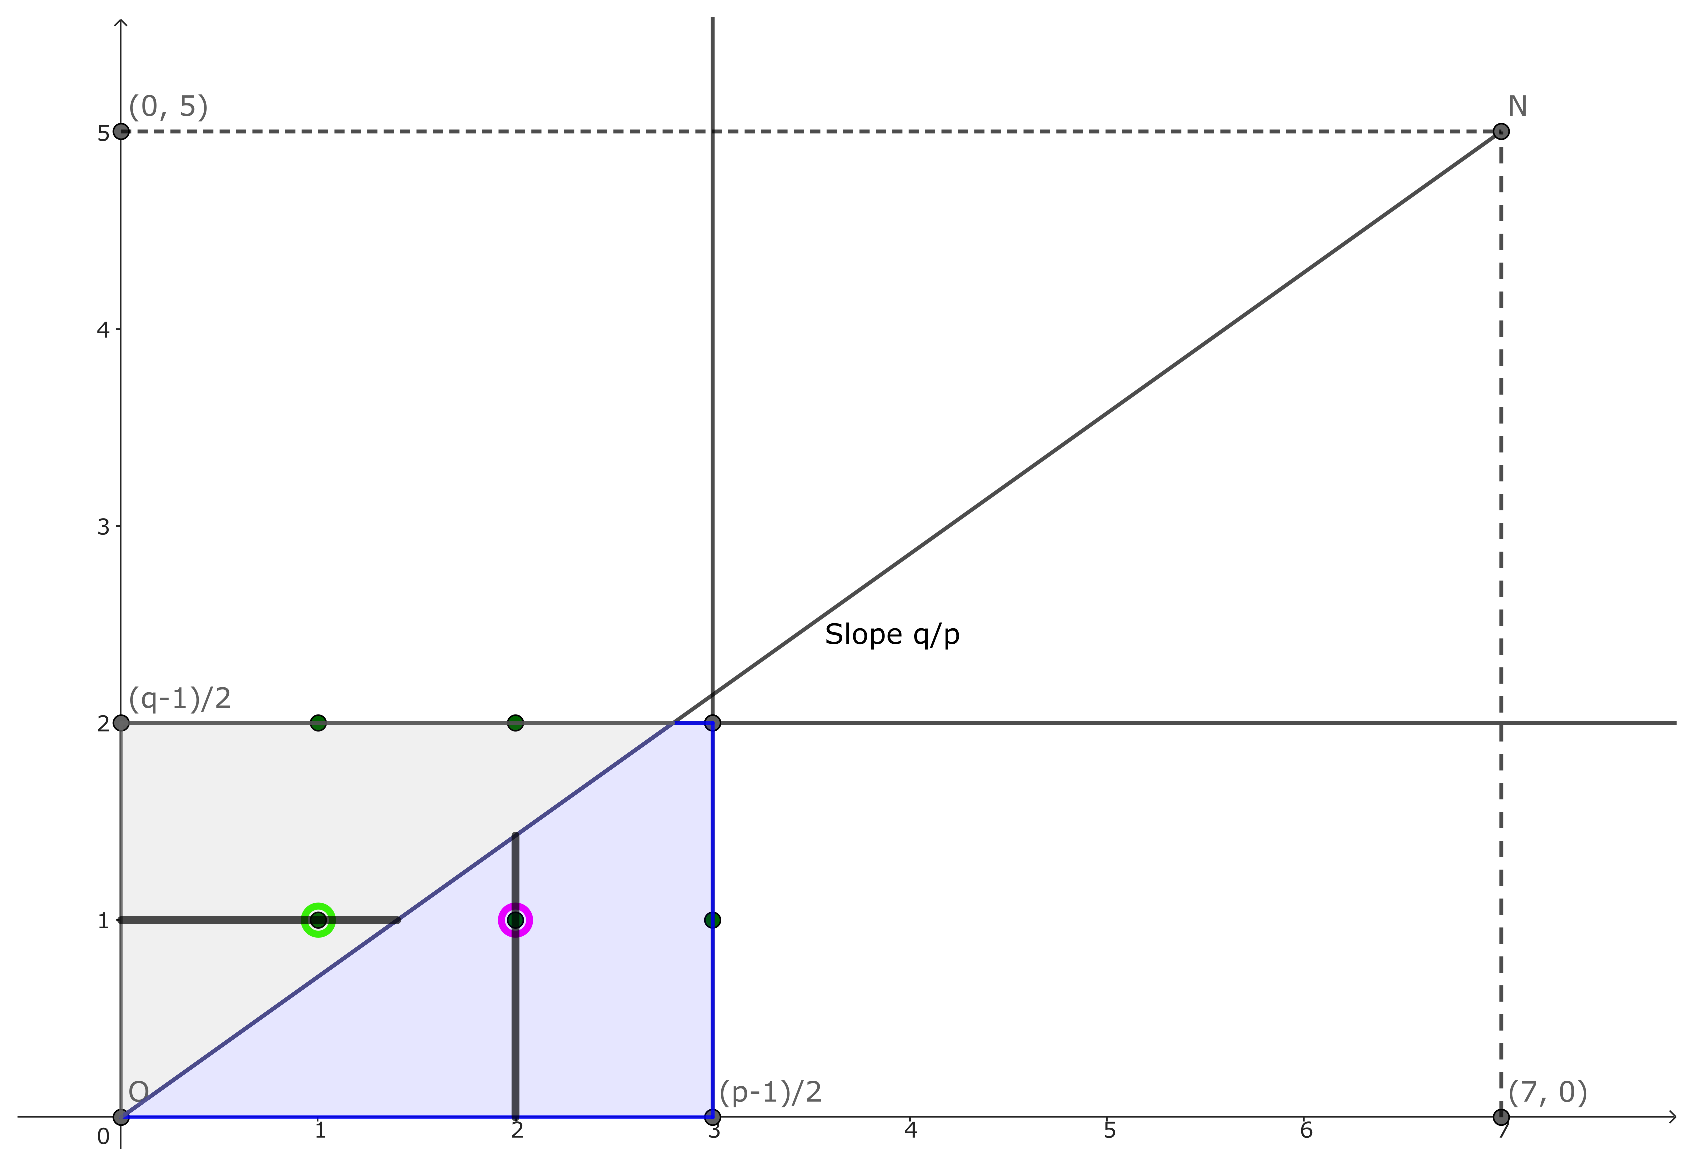
\includegraphics[width=.7\textwidth]{../otherDocuments/Lattice75}
                \caption{The lattice for the $p=7, q=5$ problem, with the $j=1$ and $k=2$ cases highlighted}\label{fig:lattice-5-7}
        \end{figure}
    }
             \begin{onlineOnly}
                Move the sliders to $p=7$ and $q=5.$
            \end{onlineOnly}
               \begin{enumerate}
                \item The line segment between the origin and $(7,5)$ has slope $\inlineAnswer[1 cm]{\tfrac{5}{7}}$. Since $p=7$ and $q=5$ are distinct primes, there are no lattice points on line segment except the endpoints.
            
                \item First, we will count the number of points $N_1$ where $\tfrac{5-1}{2}\geq y>\tfrac{5}{7}x>0.$ This triangle is grey in the GeoGebra. We will count how many lattice points on each horizontal lines $j=1,2.$ Let's just check the numbers we should get: 
                \begin{itemize}
                    \item When $j=1,$ there are $\inlineAnswer[1 cm]{1}$ lattice points.
                    \item When $j=2,$ there are $\inlineAnswer[1 cm]{2}$ lattice points.
                \end{itemize}
                For each $j$, we are counting positive integers $x<\inlineAnswer[1 cm]{\tfrac{7}{5}}j.$ Which is,
                \begin{prompt}
                    \begin{multipleChoice}
                        \choice[correct] {$\floor{\frac{7j}{5}}$}.
                        \choice {$\floor{\frac{5j}{7}}$}.
                       \end{multipleChoice}
                \end{prompt}
        
                Thus, the total number of lattice points in this triangle, $N_1,$ is 
                \begin{prompt}
                    \begin{multipleChoice}
                        \choice[correct] {$N_1=\sum_{j=1}^{2}\floor{\frac{7j}{5}}$}
                        \choice {$N_1=\sum_{j=1}^{2}\floor{\frac{5j}{7}}$}
                        \choice {$N_1=\sum_{j=1}^{3}\floor{\frac{7j}{5}}$}
                        \choice {$N_1=\sum_{j=1}^{3}\floor{\frac{5j}{7}}$}
                       \end{multipleChoice}
                \end{prompt}
        
                \item Next we will count the rest of the lattice points in the rectangle, the blue region in the GeoGebra. We willl call this number $N_2$.
                
                The region is bounded by $0<x\leq \tfrac{7-1}{2},$ $0<y<\tfrac{5}{7}x,$ and $y\leq \tfrac{5-1}{2}.$ Now, the point $A$ where $y=\tfrac{5}{7}x$ intersects $y=\tfrac{5-1}{2}$ is between two consecutive lattice points, with coordinates 
                \begin{prompt}
                    $x=\inlineAnswer[1 cm]{2}, y=\inlineAnswer[1 cm]{2}$ and $x=\inlineAnswer[1 cm]{3}, y=\inlineAnswer[1 cm]{2}.$
                \end{prompt}
                Similarly, the point $B$ where $y=\tfrac{5}{7}x$ intersects $x=\tfrac{7-1}{2}$ is between two consecutive lattice points, with coordinates 
                \begin{prompt}
                    $x=\inlineAnswer[1 cm]{3}, y=\inlineAnswer[1 cm]{2}$ and $x=\inlineAnswer[1 cm]{3}, y=\inlineAnswer[1 cm]{3}.$
                \end{prompt}
                Thus, the only lattice point in the triangle $A,B$ and $\left(\tfrac{7-1}{2},\tfrac{5-1}{2}\right)$ is $\left(\tfrac{7-1}{2},\tfrac{5-1}{2}\right)$. Therefore, there are also $N_2$ lattice points in the triangle with vertices $(0,0), \left(\tfrac{7-1}{2},0\right), \left(\tfrac{7-1}{2},\tfrac{5-1}{2}\right).$
                
                \item We use the same method as $N_1$ to find $N_2.$ We will count how many lattice points on each vertical lines $k=1,2,3.$ Let's just check the numbers we should get: 
                \begin{itemize}
                    \item When $k=1,$ there are $\inlineAnswer[1 cm]{0}$ lattice points.
                    \item When $k=2,$ there are $\inlineAnswer[1 cm]{1}$ lattice points.
                    \item When $k=3,$ there are $\inlineAnswer[1 cm]{2}$ lattice points.
                \end{itemize}
                For each $k$, we are counting positive integers $y<\inlineAnswer[1 cm]{\tfrac{5}{7}}k.$ Which is,
                \begin{prompt}
                    \begin{multipleChoice}
                        \choice {$\floor{\frac{7j}{5}}$}.
                        \choice[correct] {$\floor{\frac{5j}{7}}$}.
                       \end{multipleChoice}
                \end{prompt}
        
                Thus, the total number of lattice points in this triangle is 
                \begin{prompt}
                    \begin{multipleChoice}
                        \choice {$N_2=\sum_{k=1}^{2}\floor{\frac{7k}{5}}$}
                        \choice {$N_2=\sum_{k=1}^{2}\floor{\frac{5k}{7}}$}
                        \choice {$N_2=\sum_{k=1}^{3}\floor{\frac{7k}{5}}$}
                        \choice[correct] {$N_2=\sum_{k=1}^{3}\floor{\frac{5k}{7}}$}
                       \end{multipleChoice}
                \end{prompt}
           \end{enumerate}
            
           Thus, the total number of lattice points is $N_1+N_2=\inlineAnswer{(3)(2)}.$	
        \end{br}
             
	
\begin{br}
	The steps below outline the proof in the general case, when $p=23$ and $q=13$.
	\pdfOnly{
	\begin{figure}[h]
		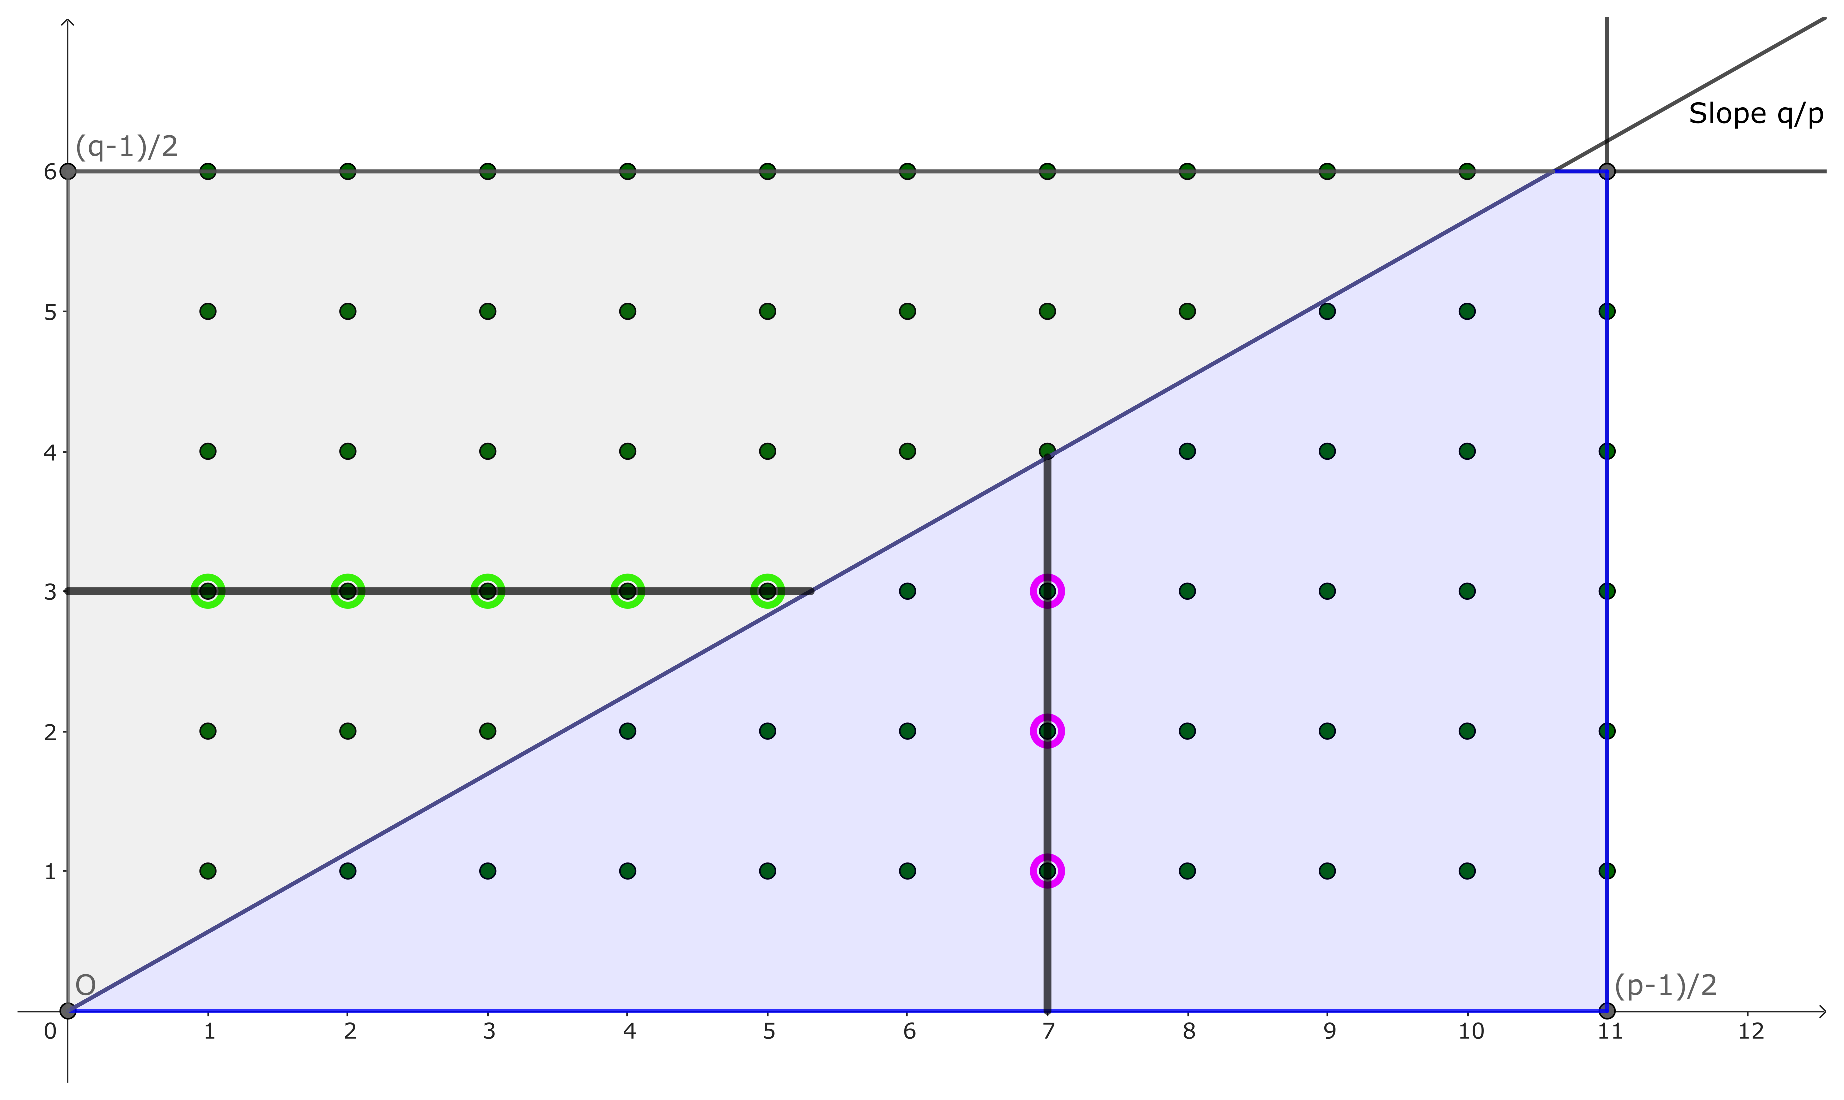
\includegraphics[width=.7\textwidth]{../otherDocuments/Lattice2313}
		\caption{The lattice for the $p=23, q=13,$ with the $j=3$ and $k=7$ cases highlighted}\label{fig:lattice-23-13}
	\end{figure}
	}
		\begin{onlineOnly}
		Move the sliders to $p=23$ and $q=13.$
	\end{onlineOnly}
		\begin{enumerate}
		\item The line segment between the origin and $(23,13)$ has slope $\inlineAnswer[1 cm]{\tfrac{13}{23}}$. Since $p=23$ and $q=13$ are distinct primes, there are no lattice points on line segment except the endpoints.
	
		\item First, we will count the number of points $N_1$ where $\tfrac{13-1}{2}\geq y>\tfrac{13}{23}x>0.$ This triangle is grey in the GeoGebra. We will count how many lattice points on each horizontal lines $j=1,2,\dots,\inlineAnswer[1 cm]{6}.$ 
		Let's just check one case, we should get: 
		\begin{itemize}
			\item When $j=3,$ \pdfOnly{as in \autoref{fig:lattice-23-13},} there are $\inlineAnswer[1 cm]{5}$ lattice points.
		\end{itemize}
		For each $j$, we are counting positive integers $x<\inlineAnswer[1 cm]{\tfrac{23}{13}}j.$ Which is,
		\begin{prompt}
			\begin{multipleChoice}
				\choice[correct] {$\floor{\frac{23j}{13}}$}.
				\choice {$\floor{\frac{13j}{23}}$}.
				\end{multipleChoice}
		\end{prompt}

		Thus, the total number of lattice points in this triangle is 
		\begin{prompt}
			\begin{multipleChoice}
				\choice[correct] {$N_1=\sum_{j=1}^{6}\floor{\frac{23j}{13}}$}
				\choice {$N_1=\sum_{j=1}^{6}\floor{\frac{13j}{23}}$}
				\choice {$N_1=\sum_{j=1}^{11}\floor{\frac{23j}{13}}$}
				\choice {$N_1=\sum_{j=1}^{11}\floor{\frac{13j}{23}}$}
				\end{multipleChoice}
		\end{prompt}

		\item Next we will count the rest of the lattice points in the rectangle, the blue region in the GeoGebra. We willl call this number $N_2$.
		
		The region is bounded by $0<x\leq \tfrac{23-1}{2},$ $0<y<\tfrac{13}{23}x,$ and $y\leq \tfrac{13-1}{2}.$ Now, the point $A$ where $y=\tfrac{13}{23}x$ intersects $y=\tfrac{13-1}{2}$ is between two consecutive lattice points, with coordinates 
		\begin{prompt}
			$x=\inlineAnswer[1 cm]{10}, y=\inlineAnswer[1 cm]{6}$ and $x=\inlineAnswer[1 cm]{11}, y=\inlineAnswer[1 cm]{6}.$
		\end{prompt}
		Similarly, the point $B$ where $y=\tfrac{13}{23}x$ intersects $x=\tfrac{23-1}{2}$ is between two consecutive lattice points, with coordinates 
		\begin{prompt}
			$x=\inlineAnswer[1 cm]{11}, y=\inlineAnswer[1 cm]{6}$ and $x=\inlineAnswer[1 cm]{11}, y=\inlineAnswer[1 cm]{7}.$
		\end{prompt}
		Thus, the only lattice point in the triangle $A,B$ and $\left(\tfrac{23-1}{2},\tfrac{13-1}{2}\right)$ is $\left(\tfrac{23-1}{2},\tfrac{13-1}{2}\right)$. Therefore, there are also $N_2$ lattice points in the triangle with vertices $(0,0), \left(\tfrac{23-1}{2},0\right), \left(\tfrac{23-1}{2},\tfrac{13-1}{2}\right).$
		
		\item We use the same method as $N_1$ to find $N_2.$ We will count how many lattice points on each vertical lines $k=1,2,\dots,\inlineAnswer[1 cm]{11}.$ Let's just check the numbers we should get: 
		\begin{itemize}
			\item When $k=7,$ \pdfOnly{as in \autoref{fig:lattice-23-13},} there are $\inlineAnswer[1 cm]{3}$ lattice points.
		\end{itemize}
		For each $k$, we are counting positive integers $y<\inlineAnswer[1 cm]{\tfrac{13}{23}}k.$ Which is,
		\begin{prompt}
			\begin{multipleChoice}
				\choice {$\floor{\frac{23j}{13}}$}.
				\choice[correct] {$\floor{\frac{13j}{23}}$}.
				\end{multipleChoice}
		\end{prompt}

		Thus, the total number of lattice points in this triangle is 
		\begin{prompt}
			\begin{multipleChoice}
				\choice {$N_2=\sum_{k=1}^{6}\floor{\frac{23k}{13}}$}
				\choice {$N_2=\sum_{k=1}^{6}\floor{\frac{13k}{23}}$}
				\choice {$N_2=\sum_{k=1}^{11}\floor{\frac{23k}{13}}$}
				\choice[correct] {$N_2=\sum_{k=1}^{11}\floor{\frac{13k}{23}}$}
				\end{multipleChoice}
		\end{prompt}
		\end{enumerate}
	
		Thus, the total number of lattice points is $N_1+N_2=\inlineAnswer{(11)(6)}.$	
\end{br}


Now we will use without proof that 
\begin{lemma}\label{lem:count-points-qr}
	Let $p$ be an odd prime number and let $a\in\mathbb{Z}$ with $p\nmid a$ and $a$ odd. If \[N=\sum_{j=1}^{\frac{p-1}{2}}\floor{\frac{ja}{p}},\] then \[\left(\frac{a}{p}\right)=(-1)^N.\]
\end{lemma}

\begin{proof}[Proof of \nameref{quad-rec-standard-form}]
	Let $p$ and $q$ be distinct odd primes. Then from \nameref{lem:count-points-qr}, 
	\[
		\legendre{p}{q}=(-1)^{N_1},\quad \legendre{q}{p}=(-1)^{N_2}, 
		\qquad \textnormal{where}\quad 
		N_1=\sum_{j=1}^{\frac{q-1}{2}}
		\floor{\frac{p}{q}j}
		\quad \textnormal{and}\quad 
		N_2=\sum_{j=1}^{\frac{p-1}{2}}\floor{\frac{q}{p}j}.
	\]
	Thus, $\legendre{p}{q}\legendre{q}{p}=(-1)^{N_1+N_2}.$ It remains to show that $N_1+N_2=\left(\frac{p-1}{2}\right)\left(\frac{q-1}{2}\right).$

	Without loss of generality, assume that $p>q$. We draw the rectangle $(0,0), \left(\tfrac{p-1}{2},0\right), \left(\tfrac{p-1}{2},\tfrac{q-1}{2}\right),$ and $\left(0,\tfrac{q-1}{2}\right)$, as in the GeoGebra example. Then there are $\left(\frac{p-1}{2}\right)\left(\frac{q-1}{2}\right)$ lattice points in this rectangle, excluding the axes.
	
	The line segment between the origin and $(p,q)$ has slope $\answer{\tfrac{q}{p}}$. Since $p$ and $q$ are distinct primes, there are no lattice points on line segment except the endpoints.
	

	For each $j$, we are counting positive integers $x<\answer{\tfrac{p}{q}}j.$ Which is,
		\begin{prompt}
			\begin{multipleChoice}
				\choice[correct] {$\floor{\frac{pj}{q}}$}.
				\choice {$\floor{\frac{qj}{p}}$}.
			   \end{multipleChoice}
		\end{prompt}

	Thus, the total number of lattice points in this triangle is 
		\begin{prompt}
			\begin{multipleChoice}
				\choice[correct] {$N_1=\sum_{j=1}^{(q-1)/2}\floor{\frac{pj}{q}}$}
				\choice {$N_1=\sum_{j=1}^{(q-1)/2}\floor{\frac{qj}{p}}$}
				\choice {$N_1=\sum_{j=1}^{(p-1)/2}\floor{\frac{pj}{q}}$}
				\choice {$N_1=\sum_{j=1}^{(p-1)/2}\floor{\frac{qj}{p}}$}
   			\end{multipleChoice}
		\end{prompt}

	Next we will count the rest of the lattice points in the rectangle, the blue region in the GeoGebra. We willl call this number $N_2$.
	The region is bounded by $0<x\leq \tfrac{p-1}{2},$ $0<y<\tfrac{q}{p}x,$ and $y\leq \tfrac{q-1}{2}.$ Now, the point $A$ where $y=\tfrac{q}{p}x$ intersects $y=\tfrac{q-1}{2}$ is between two consecutive lattice points, with coordinates 
		\begin{prompt}
			$x=\answer{10}, y=\answer{(q-1)/2}$ and $x=\answer{(p-1)/2}, y=\answer{(q-1)/2}.$
		\end{prompt}
	Similarly, the point $B$ where $y=\tfrac{q}{p}x$ intersects $x=\tfrac{p-1}{2}$ is between two consecutive lattice points, with coordinates 
		\begin{prompt}
			$x=\answer{(p-1)/2}, y=\answer{(q-1)/2}$ and $x=\answer{(p-1)/2}, y=\answer{7}.$
		\end{prompt}
	Thus, the only lattice point in the triangle $A,B$ and $\left(\tfrac{p-1}{2},\tfrac{q-1}{2}\right)$ is $\left(\tfrac{p-1}{2},\tfrac{q-1}{2}\right)$. Therefore, there are also $N_2$ lattice points in the triangle with vertices $(0,0), \left(\tfrac{p-1}{2},0\right), \left(\tfrac{p-1}{2},\tfrac{q-1}{2}\right).$
		
	We use the same method as $N_1$ to find $N_2.$ We will count how many lattice points on each vertical lines $k=1,2,\dots,\answer{\frac{p-1}{2}}.$ 
	For each $k$, we are counting positive integers $y<\answer{\tfrac{q}{p}}k.$ Which is,
		\begin{prompt}
			\begin{multipleChoice}
				\choice {$\floor{\frac{pj}{q}}$}.
				\choice[correct] {$\floor{\frac{qj}{p}}$}.
			   \end{multipleChoice}
		\end{prompt}

	Thus, the total number of lattice points in this triangle is 
		\begin{prompt}
			\begin{multipleChoice}
				\choice {$N_2=\sum_{k=1}^{(q-1)/2}\floor{\frac{pk}{q}}$}
				\choice {$N_2=\sum_{k=1}^{(q-1)/2}\floor{\frac{qk}{p}}$}
				\choice {$N_2=\sum_{k=1}^{(p-1)/2}\floor{\frac{pk}{q}}$}
				\choice[correct] {$N_2=\sum_{k=1}^{(p-1)/2}\floor{\frac{qk}{p}}$}
   			\end{multipleChoice}
		\end{prompt}

	Thus, the total number of lattice points is $N_1+N_2=\sum_{k=1}^{(q-1)/2}\floor{\frac{pk}{q}}+\sum_{k=1}^{(p-1)/2}\floor{\frac{qk}{p}}=\left(\frac{p-1}{2}\right)\left(\frac{q-1}{2}\right)$
\end{proof}
	
\bibliographystyle{apalike}
\bibliography{sources}


\end{document}
